% !TeX root = RJwrapper.tex
\title{Conversations in time: interactive visualisation to explore
structured temporal data}
\author{by Earo Wang, Dianne Cook}

\maketitle

\abstract{%
An abstract of less than 150 words.
}

\hypertarget{introduction}{%
\section{Introduction}\label{introduction}}

\begin{itemize}
\tightlist
\item
  An ensemble of graphics
\item
  Accelerate the exploratory data visualization process
\end{itemize}

\hypertarget{background-tidy-temporal-data-and-workflow}{%
\section{Background: tidy temporal data and
workflow}\label{background-tidy-temporal-data-and-workflow}}

The \CRANpkg{tsibble} package \citep{wang2020tsibble} introduces a
unified temporal data structure, referred to as a \texttt{tsibble}, to
represent time series and longitudinal data in a tidy format
\citep{wickham2014tidy}. That said, a \texttt{tsibble} extends the
\texttt{data.frame} and \CRANpkg{tibble} class with temporally
contextual metadata: \texttt{index} and \texttt{key}. The \texttt{index}
declares a data column that holds time-related indices. The \texttt{key}
identifies a collection of related series or panels observed over the
\texttt{index}-defined period, which can comprise multiple columns.
Below displays the monthly Australian retail trade turnover data
(\texttt{aus\_retail}), available in the \CRANpkg{tsibbledata} package.
The \texttt{Month} column holds year-months as \texttt{index}. The
\texttt{State} together with \texttt{Industry} are the identifiers for
these 152 series, highlighted as \texttt{key}. Note that the column
\texttt{Series\ ID} could be an alternative option for setting up
\texttt{key}, but \texttt{State} and \texttt{Industry} are more readable
and informative. The \texttt{index} and \texttt{key} are ``sticky''
columns to a \texttt{tsibble}, forming critical pieces for fluent
temporal data analysis later.

\begin{Schunk}
\begin{Soutput}
#> # A tsibble: 64,532 x 5 [1M]
#> # Key:       State, Industry [152]
#>   State                Industry                    `Series ID`    Month Turnover
#>   <chr>                <chr>                       <chr>          <mth>    <dbl>
#> 1 Australian Capital ~ Cafes, restaurants and cat~ A3349849A   1982 Apr      4.4
#> 2 Australian Capital ~ Cafes, restaurants and cat~ A3349849A   1982 May      3.4
#> 3 Australian Capital ~ Cafes, restaurants and cat~ A3349849A   1982 Jun      3.6
#> 4 Australian Capital ~ Cafes, restaurants and cat~ A3349849A   1982 Jul      4  
#> 5 Australian Capital ~ Cafes, restaurants and cat~ A3349849A   1982 Aug      3.6
#> # ... with 64,527 more rows
\end{Soutput}
\end{Schunk}

In the spirit of tidy data to the \CRANpkg{tidyverse}
\citep{Wickham2019}, the \textbf{tidyverts} suite features
\texttt{tsibble} as the foundational data structure, in order to build a
fluid and fluent pipeline for time series analysis. Besides
\CRANpkg{tsibble}, the \CRANpkg{feasts} and \CRANpkg{fable} packages
fill the role of statistical analysis and forecasting in the
\textbf{tidyverts} ecosystem. When time series analysis starts taking
off, series of interest denoted by the \texttt{key} variables often
remain unchanged over the course of analysis, from trend inspection to
forecasting performance.

Figure \ref{fig:highlight-retail} (a) gives an overview of 152 series
for the retail data using an overlaid time series plot, while Figure
\ref{fig:highlight-retail} (b) presents a scatterplot, where each series
is represented by a dot in the feature space (trend versus seasonal
strength). The plot making of Figure \ref{fig:highlight-retail} (b) is
aided with the \texttt{features()} function from \CRANpkg{feasts}, which
summarises original data by each series down to various statistical
features. This function along with other \textbf{tidyverts} functions is
\texttt{tsibble}-aware, and outputs a table in a reduced form where each
row corresponds to a series, thus graphically displayed as Figure
\ref{fig:highlight-retail} (b).

\begin{Schunk}
\begin{figure}

{\centering 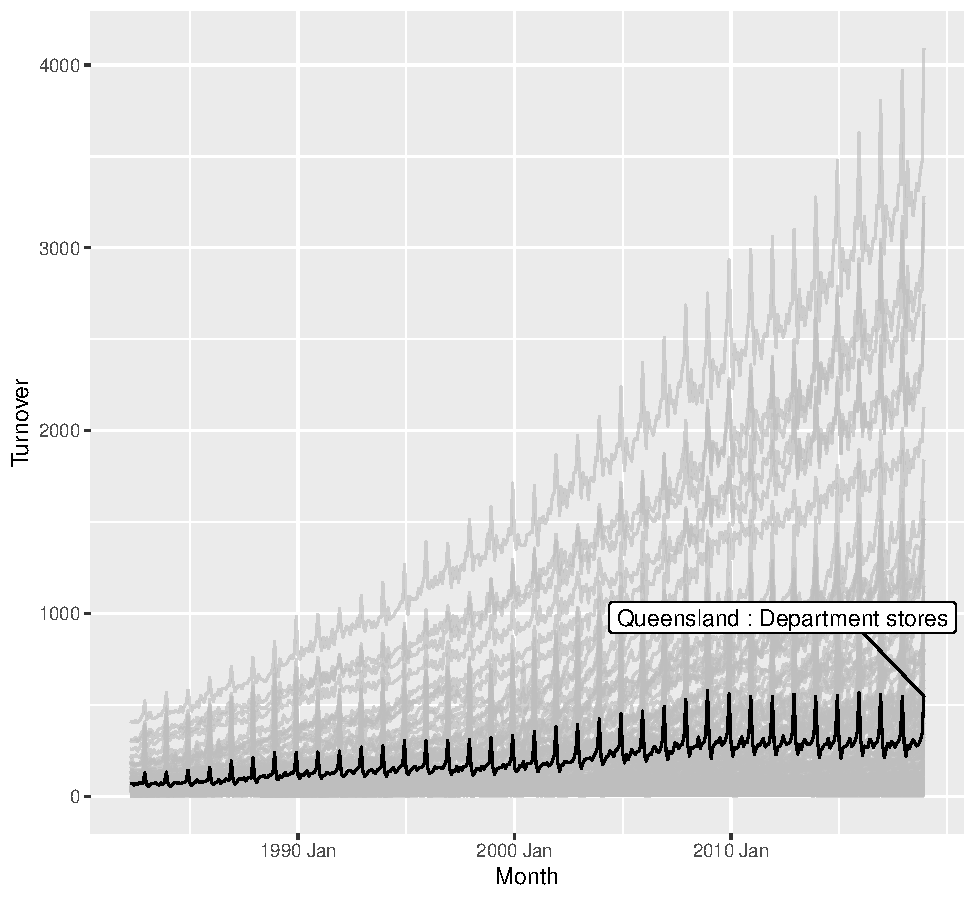
\includegraphics[width=\textwidth]{figure/highlight-retail-1} 

}

\caption[ToDo]{ToDo}\label{fig:highlight-retail}
\end{figure}
\end{Schunk}

Figure \ref{fig:highlight-retail} highlights not only a series with
strongest seasonality, but also a need to querying interesting series on
the fly. Without interactivity, one needs to first filter the
interesting series out from the features table, and join back to the
original \texttt{tsibble} in order to examine its trend in relation to
others. This procedure can soon grow cumbersome if many series to be
discovered. Despite that the two plots are static, they can be
considered as linked views via the common \texttt{key} variables between
two tables. This motivates enabling interactivity of \texttt{tsibble}
and \texttt{tsibble}-derived objects for rapid exploratory data
analysis.

\hypertarget{overview-of-interactivity}{%
\section{Overview of interactivity}\label{overview-of-interactivity}}

\begin{itemize}
\tightlist
\item
  \{cranvas\} and \{cranvastime\}
\item
  \href{http://crossfilter.github.io/crossfilter/}{crossfilter.js} \&
  \href{https://dc-js.github.io/dc.js/}{dc.js}
\item
  \{crosstalk\} and html widgets
\item
  \{rJava\}, \{rbokeh\} \{loon\}
\end{itemize}

\hypertarget{interactivity-for-coordinated-views-via-shared-temporal-data}{%
\section{Interactivity for coordinated views via shared temporal
data}\label{interactivity-for-coordinated-views-via-shared-temporal-data}}

The \CRANpkg{tsibbletalk} package, inspired by the \CRANpkg{crosstalk}
package, introduces a shared tsibble data structure on top of a
\texttt{tsibble} to allow for frictionless communication between
different plots for temporal data. The \texttt{as\_shared\_tsibble()}
function provides an entry point in the integrated flow, turning a
\texttt{tsibble} to a shared instance (i.e.~\texttt{SharedTsibbleData}
subclassing of \texttt{SharedData} from \CRANpkg{crosstalk}) that powers
data transmission across multiple views. The \CRANpkg{tsibbletalk}
package aims to streamline interactive graphical analysis with the focus
of temporal and structured linking.

As opposed to one-to-one linking, \CRANpkg{tsibbletalk} defaults to
categorical linking where marking one or more observations in one
category will broadcast to all other observations in this category.
Given time series plots, click any data point on a line, highlighting
the whole line as a result. The \texttt{as\_shared\_tsibble()} uses
\texttt{tsibble}'s \texttt{key} variables to achieve these types of
linking, and the \texttt{spec} argument takes one step further in
constructing hybrid linking, such as hierarchical and categorical
linking. For example, each series in the \texttt{aus\_retail} data
corresponds to all possible combinations of the \texttt{State} and
\texttt{Industry} variables. They are intrinsically crossed with each
other. If one variable is nested within another, this lends itself to a
hierarchical structure, like geographical hierarchy. Such collection of
inter-related time series are referred to as hierarchical and grouped
time series in the literature \citep{fpp}.

To incorporate structured specifications in the \texttt{key}, a symbolic
formula can be passed to the \texttt{spec} argument. Adopting Wilkinson
notations for factorial models \citep{Wilkinson1973}, the \texttt{spec}
follows the \texttt{/} and \texttt{*} operators tradition to declare
nesting and crossing variables respectively. The \texttt{spec} for the
\texttt{aus\_retail} data is therefore specified as
\texttt{State\ *\ Industry} or \texttt{Industry\ *\ State}, which is the
default for the presence of multiple \texttt{key} variables. If there is
a hierarchy in the data, using \texttt{/} is required to indicate the
parent-child relation, as strictly one direction \texttt{parent/child}.

The \texttt{tourism\_monthly} dataset packaged in \CRANpkg{tsibbletalk},
contains monthly domestic overnight trips across Australia, to give an
illustrator of nesting and crossing. The \texttt{key} is comprised of
three identifying variables: \texttt{State}, \texttt{Region}, and
\texttt{Purpose} (of trip), in particular \texttt{State} nesting of
\texttt{Region}, together crossed with \texttt{Purpose}. This
specification can be translated as follows:

\begin{Schunk}
\begin{Sinput}
library(tsibbletalk)
tourism_shared <- tourism_monthly %>% 
  as_shared_tsibble(spec = (State / Region) * Purpose)
\end{Sinput}
\end{Schunk}

This dataset contains a three-level hierarchy: the root node is
implicitly Australia, and geographically disaggregated to states and
lower-level tourism regions. A new handy function
\texttt{plotly\_key\_tree()} has been implemented to address the need of
hierarchical discovery arising from the data. It interprets hierarchies
in the shared tsibble's \texttt{spec} as a tree view, built with
\CRANpkg{plotly}. The following code line produces the linked tree
diagram and fills the left panel of Figure
\ref{fig:tourism-linking-fig}. The visual of tree hierarchy untangles a
group of related series and snapshots the data organisation from a
bird's eye view.

\begin{Schunk}
\begin{Sinput}
p_l <- plotly_key_tree(tourism_shared, height = 1100, width = 800)
\end{Sinput}
\end{Schunk}

The tree plot provides backbones of the data, and much flesh yet to be
attached. Small multiples of time series lines are composed and placed
at the top right of Figure \ref{fig:tourism-linking-fig} to unpack the
temporal trend across regions by purposes of trips. The shared tsibble
data can be directly piped into \CRANpkg{ggplot2} code.

\begin{Schunk}
\begin{Sinput}
p_tr <- tourism_shared %>%
  ggplot(aes(x = Month, y = Trips)) +
  geom_line(aes(group = Region), alpha = .5, size = .4) +
  facet_wrap(~ Purpose, scales = "free_y") +
  scale_x_yearmonth(date_breaks = "5 years", date_labels = "%Y")
\end{Sinput}
\end{Schunk}

To tease apart these overlaid time series, they are funnelled through
the \texttt{features()} S3 method to extract some key characteristics,
including the measurements of trend and seasonality. A scatterplot is
populated from these statistics for each series.

\begin{Schunk}
\begin{Sinput}
tourism_feat <- tourism_shared %>%
  features(Trips, feat_stl)
p_br <- tourism_feat %>%
  ggplot(aes(x = trend_strength, y = seasonal_strength_year)) +
  geom_point(aes(group = Region))
\end{Sinput}
\end{Schunk}

Lastly, three graphics are composed as an ensemble of coordinated views
for multi-facetted exploration, shown as Figure
\ref{fig:tourism-linking-fig} (the interactive realisation of Figure
\ref{fig:highlight-retail}). Routine functions bring about new
interaction with temporal data on the client side (i.e.~without Shiny).

\begin{Schunk}
\begin{Sinput}
subplot(p_l,
  subplot(
    ggplotly(p_tr, tooltip = "Region", width = 1100),
    ggplotly(p_br, tooltip = "Region", width = 1100),
    nrows = 2),
  widths = c(.4, .6)) %>%
  highlight(dynamic = TRUE)
\end{Sinput}
\end{Schunk}

Since all plots are stemmed from one shared tsibble data source, they
are self-linking views. Nodes, lines, and points are clickable. For
example, selecting the leaf node ``Melbourne'' fires up four respective
series of the \texttt{Purpose} category in other subplots, characterised
by ``categorical linking''. Press the ``Shift'' key to switch on
persistent selection, and simultaneously select the parent node
``Western Australia'' to trigger its children. The domestic tourism
performance in Melbourne can be quickly compared against the whole state
of Western Australia. It makes navigation simpler than conditional
panels, and also enables persistent selection for comparisons across
groups.

\begin{Schunk}
\begin{figure}

{\centering 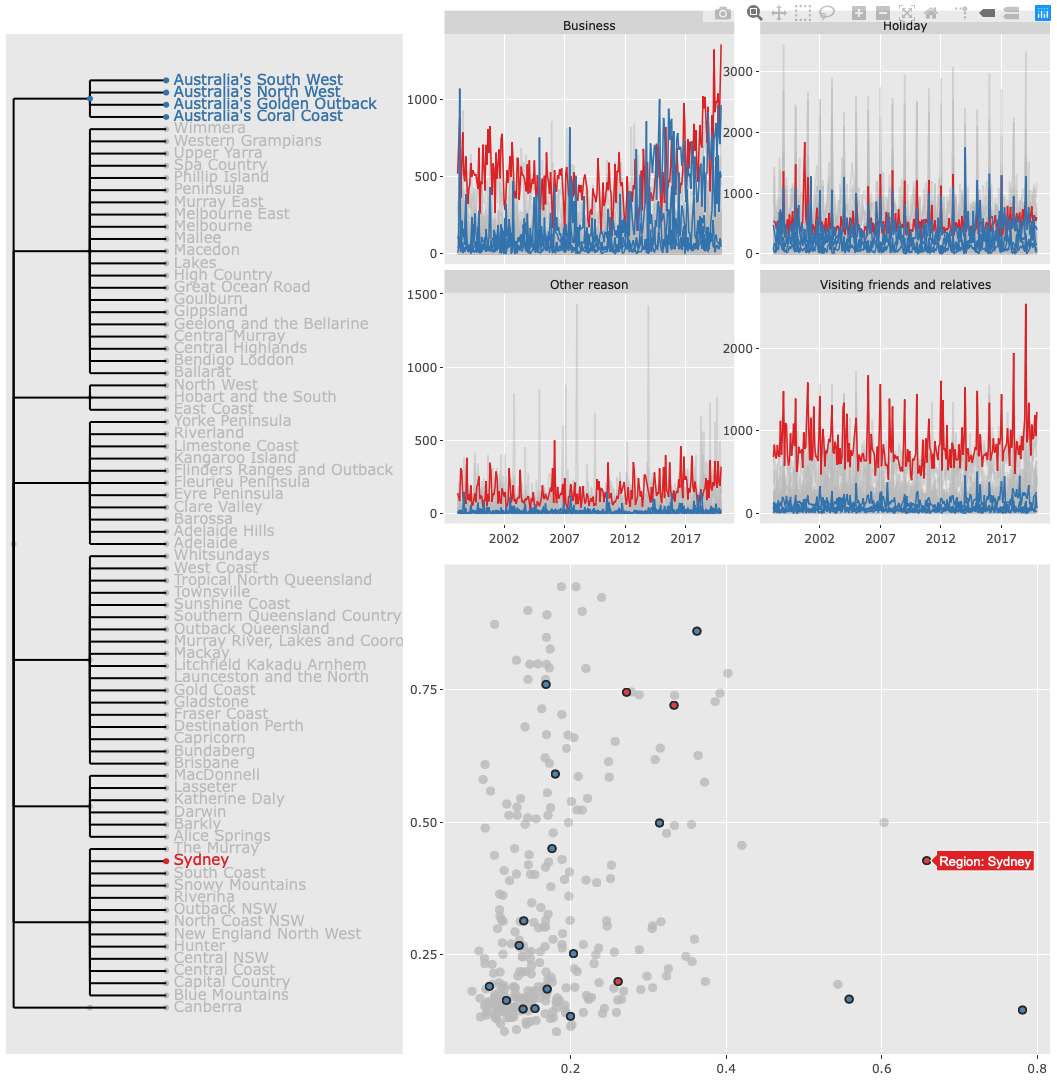
\includegraphics[width=\textwidth]{img/tourism-linking} 

}

\caption[ToDo]{ToDo}\label{fig:tourism-linking-fig}
\end{figure}
\end{Schunk}

\hypertarget{slicing-and-dicing-time}{%
\section{Slicing and dicing time}\label{slicing-and-dicing-time}}

The other critical aspect of a tsibble is ``index'', that provides
foundational temporal context. A common tool in time series analytical
toolkit is seasonal plots that lay time series not on the whole time
scale, but on an origin-less relative time unit, for example
\texttt{gg\_season()} in the \{feasts\} package. It helps to examine and
emphasise periodic/aperiodic patterns, comparing to time series plots
that primarily focus on trends. Standard seasonal plots break the
overall time into two components: seasonal periods on the x-axis, and
grouped by their corresponding lower-resolution time. For example,
monthly data can be decomposed into months separated by years, and
hourly data into hours grouped by days. Data collected at lower-level
resolutions often exhibits more than one seasonal patterns. To discover
typical seasonal or non-typical profiles, it is helpful to quickly
browse through many possible periods. Interactivity ought to be enabled.

The \{tsibbletalk\} package provides a pair of UI and server functions,
as a shiny module, to help with finding interesting time slices in a
shiny application. The pair, decoupled to \texttt{tsibbleDiceUI()} and
\texttt{tsibbleDiceServer()}, presents a clean interface and forms a
resusable piece. Like all shiny modules, users should supply a unique
session id. The UI function \texttt{tsibbleDiceUI()} shows a slider that
controls the number of periods, and a plot specified by users. The
server function \texttt{tsibbleDiceServer()} is the workhorse,
transforming data and updating the plot. It expects a \texttt{ggplot}
(converted to \texttt{plotly} via \texttt{ggplotly()}) or
\texttt{plotly} object. This plot can be line charts, or other graphical
elements (such as boxplots). But it assumes that tsibble's time index is
plotted on the x-axis. The other mandatory argument is to specify the
number of seasonal periods that requires shifting.

(Data flows) Transformed data generally requires redrawing the plot, and
worsen the performance of shiny. The underlying tsibble data is called
back and transformed in R. Using the \texttt{plotly.js} react method,
only transformed data is sent to the server side, while keeping the rest
configuration unchanged (e.g.~layout and graphical elements). It is
performant, and users will not experience notable delay in response to
the change in the slider input. Dissect time index, and propagate
transformed data to shiny server.

\hypertarget{conclusions-and-discussions}{%
\section{Conclusions and
discussions}\label{conclusions-and-discussions}}

\bibliography{references.bib}

\address{%
Earo Wang\\
The University of Auckland\\
Department of Statistics\\ The University of Auckland\\ New Zealand\\
}
\href{mailto:earo.wang@auckland.ac.nz}{\nolinkurl{earo.wang@auckland.ac.nz}}

\address{%
Dianne Cook\\
Monash University\\
Department of Econometrics and Business Statistics\\ Monash
University\\ Australia\\
}
\href{mailto:dicook@monash.edu}{\nolinkurl{dicook@monash.edu}}
